\documentclass[letterpaper,10pt]{article}
\usepackage{biblatex} %Imports biblatex package
\addbibresource{references.bib} %Import the bibliography file
\usepackage{graphicx} % Required for inserting images
\usepackage{float}

\title{What strategies makes alpine ski racers perform well on flats in slalom and what is a good training strategy to learn these strategies}
\author{Christian Magelssen}
\date{January 2024}

\begin{document}

\maketitle

\section{Background}

In alpine ski racing, the goal is to ski a slalom course in the shortest time possible. Descents can be executed in nearly any way, as long as the athlete passes on the correct side of the gates placed along the slope. This aspect introduces a significant degree of freedom in technique selection. To address this freedom of choice, researchers have sought to identify the strategies and techniques employed by athletes to tackle this challenge.

Understanding these strategies is crucial knowledge for coaches to enhance their training practices. It helps coaches identify which techniques and strategies may be beneficial to emphasize in training sessions. However, a key challenge in this research is the diverse nature of alpine skiing situations. Principles derived from one scenario may not necessarily apply to another. This highlights the need for a nuanced approach, recognizing that what works in one situation may not be universally applicable to others.



I alpint er målet å kjøre raskest mulig ned en løype på tid. Nedkjøringer kan gjøres på nesten alle mulige måter så lenge utøveren passerer på riktig side av porten som er plassert nedover bakken, og innbyr derfor til et stort frihetsgradsproblem. For å dette frihetsgradsproblemet har forskere forsøkt å finne ut hvilke strategier og teknikker utøvere bruker for å løse dette frihetsgradsproblemet. Dette er viktig kunnskap som trenere kan bruke i sin trenerpraksis, som å vite hvilke teknikker og strategier det kan være fornuftig å stimulere til i treningsarbeidet. En utfordring med dette arbeidet er at situasjonene i alpint er svært forskjellige, slik prinsipper fra en situasjonen ikke nødvendigvs gjelder en annen. Det betyr 


. Derfor har forskere forsøkt å studere hvilke mekanismer som er lagt til grunn for dette arbeidet. En utfordring med dette arbeidet er at situasjonene i alpint, som betyr at det vanskelig å studere noe i en situasjon. Derfor er det viktig å belyse teknikk, men det er like mye 

Det ekspert performance approach er en teoretisk tilnærming som omhandler hvordan gir et teoretisk rammeverk for å studere alpint. Rammeverket går ut på. Med utgangspunkt i dette teoretiske rammeverket har denne studien forsøkt å finne ut hva som er en. Vi fokuserer på tekniske ferdigheter.

\section{Introduction}


\subsection{What distinguishes skilled performers from less skilled performers?}

The first step in the expert performance approach is to capture differences that discriminate between the best and less skilled performers in alpine skiing. Then, to design representative tasks that allow experts to reproduce their superiority.

Alpine ski racers often compete with small time differentials in completing a slalom course. For instance, in a slalom race, the discrepancy between the victor and the second-place finisher might be as slight as a few hundredths of a second after two runs on a 50-second course. Despite the narrow margin in overall race time, the time gaps between skiers can be substantial when examining specific smaller segments of the slalom course. Three such crucial segments, identified through previous gate-to-gate analysis or shorter intermediate sections, are the course's hairpins, starts, and flat sections. These observations suggest that even the most skilled performers have room for improvement in particular parts of a course.

In my doctoral project, I chose to study the flat sections in a slalom course. The rationale for this choice was that the race hill in Oslo's new indoor ski hall consisted of a long, flat section that made it great for studying this skill. The skill is also more generic than the hairpin and the start since the flats in slalom typically cover a greater proportion of the course compared to the hairpin and the start. Moreover, an effective technique for skiing flats might also be generalized to hairpins. For these reasons, I studied the flat section in alpine ski racing. 


\subsection{How do skilled performers perform better?}
In this doctoral research project, I have chosen to study flat slopes in slalom skiing. The goal in the next phase of the expert performance approach is to identify causal mechanisms that can explain the superior performance of skilled performance in this section of the slalom course \cite{williams_using_2017}. 

From a mechanical energy perspective, the primary engine in alpine ski racing is the potential energy available to the skier at the top of the slalom course \cite{supej_differential_2008}. At the top of the slalom course, the skier has accumulated gravitational potential energy as the ski lift has exerted force against gravity to lift the skiers up to the peak. The skiers' reservoir of acquired potential energy enables the skier to perform work, such as compressing snow to initiate the ski turn. The amount of potential energy available to the skier for performing such work at the top of a slalom course can be derived from the following equation:

\[U=mgh\]
Here, U represents gravitational potential energy (measured in joules), \textit{m} represents the mass of the skier (measured in kilograms), g represents the gravitational acceleration (approximately 9.81 meters per second squared) acting on the skier, and \textit{h} represents the height (measured in metre). When the skier descends the slalom course, the amount work done by gravity can be derived by finding the gravitational potential energy for the initial position $U_1$ (at the top of the slalom course) and the gravitational potential energy for the final position $U_2$ (at the bottom of the slalom course), and then calculate the negative of change in potential energy:

\[W=-U_2 + U_1\]
\[W= -\Delta U \]
This quantity represents the work done by gravity on the skiers as they descend from the top to the bottom of the slalom course. If gravity is the only force acting on the skier, then all this work must be converted to kinetic energy to satisfy the law of conservation of mechanical energy. Kinetic energy, which represents the energy in a system due to its motion, can be derived from the following equation:

\[ K = \frac{1}{2} m v^2 \]
Here, K is the kinetic energy, m the mass of the skier and v is the velocity of the skier. Therefore, a skier with higher mass and velocity has higher kinetic energy than a lower skier and could therefore do more work, such a pushing snow. For the law of conservation of mechanical energy to hold true in a scenario where gravity is the only acting force, the sum of potential and kinetic energy (denoted as \textit{E} for mechanical energy) must remain constant during a descent: 

\[ E = U + K \]

Therefore, we can use our knowledge of the skier to calculate the speed of a skier at the bottom of the slope if the only force acting on the skier is gravity. A skier at rest at the top of the slalom course:

\[E = \frac{1}{2} m v^2_1 + mgh_1 = 0 + mgh_1\] 
At the bottom of the course, the skier has the following mechanical energy:


\[E = \frac{1}{2} m v^2_2 + mgh_2 = \frac{1}{2} m v^2_2 + 0\] 

To satisfy the law of conservation of mechanical energy, the sum of the two types of energies must constant:

\[E = \frac{1}{2} m v^2_2 = mgh_1\] 
We can therefore use the knowledge of the skiers position on the hill to calculate the speed at bottom if gravity is the sole force at play:

\[v_2 = \sqrt{2gh_1} \] 
We derive this algebraically by first cancelling the mass, and multiplying the right side of the equation by 2, and finally taking the square root of $v^2$. An example is given in fig. However, gravity is not the only force at play in alpine ski racing. A large portion of this energy dissipates to two air drag and snow friction \cite{supej_differential_2008}.


Based on principles of mechanical energy conservation is en strategi for å konserve så mye av den potensielle energi som mulig, som kan gjøres ved å kjøre carved turns instead of skidding. Dette kan gjøres ved å bruke stand against strategien, som går ut på å resist the forces down the course. 

A second way skiers can improve energy conservation is by controlling the point of attack of their center of mass along the length of the skis during a turn. When skiers shift their center of mass backward or forward in relation to the connection point with their skis (that is, binding), it directly impacts the interaction of the skis with the snow surface. For example, if a skier has edged their skis, moving the center of mass towards the tip of the ski increases friction in that area, enabling it to turn more sharply. On the other hand, if a skier has edged their skis, but shifts their center of mass backward to the skis tails, reduces the pressure of the front skis, reducing the skis pressure in the front of skis and consequently makes the turn more broadly. In ski racing, skiers want to turn more sharply in the initiation and control phases of the turn and should therefore shift their pressure shifted forward to bend the ski's forebody. However, after gate passage, skiers want to stop turning and should therefore shift their center of mass backward by rocking the skis forward. In effect, these actions can reduce snow friction and therefore energy conservation. Previous field research of elite alpine ski racers have shown that fast skiers tend to rock skis more forward and pressure the back part of the ski for considerable longer time during a turn, than slower skiers \cite{reid_kinematic_2010, tjorhom_beskrivelse_2007, reid_alpine_2020}. 

During the initiation and control phases of a turn, the pressure is generally shifted forward to bend the ski's forebody, increasing friction with the snow and enabling it to turn more sharply. However, at some point, during turn progression, the skier aims to stop turning and therefore shifts the pressure further back on the skis, thereby reducing turning and braking forces \cite{lemaster_skiers_1999, lemaster_ultimate_2010}. 

effectively enhancing the ski's ability to carve a sharper turn. 


shifted forward to bend the ski's forebody, increasing friction with the snow and enabling it to turn more sharply. 

for å forbedre konservering av energi er gjennom kontrollering av forward and backward movements. This has an effect of skis self-steering effect. During the initiation and control phases of a turn, the pressure is generally shifted forward to bend the ski's forebody, increasing friction with the snow and enabling it to turn more sharply. However, at some point, during turn progression, the skier aims to stop turning and therefore shifts the pressure further back on the skis, thereby reducing turning and braking forces \cite{lemaster_skiers_1999, lemaster_ultimate_2010}. Investigations of elite alpine ski racers have shown that high performing skiers tend to rock skis more forward and pressure the back part of the ski for considerable longer time during a turn, than slower skiers \cite{reid_kinematic_2010, tjorhom_beskrivelse_2007, reid_alpine_2020}. To make the information more specific for the skiers, we communicated, that the maximum range of the rocking movement was about 30-50 centimeters from gate passage to completion of the turn, which is in correspondence with biomechanical evidence of elite ski racers \cite{reid_kinematic_2010}. 




En tilnærming for å kjøre fortere på flater er å kjøre renere. En annen mer offensive strategi er å pumpe for å kjøre fortere på flater. I modellen til noen forskere ble. Et viktig poeng med modellen var dermed å. Et viktig element i studien var dermed å finne ut om. 

Can skiers do more than just skiing clean carved turns? One strategy to complete 







Yet, in an experiment conducted (unpublished data), our research group observed that elite skiers produced faster times in a free skiing course of gentle terrain when they made slalom turns using the pumping technique (that is, moving one’s centre of mass towards the centre of the turn) compared to straight gliding runs. This finding was an initial proof of concept that skiers could increase the velocity through muscular work by an amount larger than the potential energy was able to account for. Velocity gains exceeding the contribution of the gravitational force has also been reported in other studies4,6. For example, Reid noted that skiers sometimes achieved such effects in the transition between two slalom turns. Although there is data to support pumping as a skiing technique to increase velocity, no study has looked at the exact actions resulting in this effect. This is an important topic to study because the pumping technique has been a cornerstone in the Norwegian Ski Federation’s (NSF) technique strategy since the experiment on pumping was conducted eight years ago. Despite many efforts to improve this skill, our experience is that some skiers merit more from this technique than others but that it is difficult to pinpoint precisely what good and bad ‘pumpers’ are doing differently. Understanding the motion actions that underpin an effective pumping technique is, therefore, an important subject to study.

Owing to the importance of this skill for sporting performance for experienced and well-trained athletes, it is also critical to understand how we can optimise skill learning to enhance this skill. In experimental psychology and cognitive neuroscience, there is converging evidence showing that certain type of practices, as well as the distribution of it, contributes more effectively to the attainment of expertise than other types of practices7–10. If the effective learning paradigms discovered in this research is true, it could fundamentally alter the way coaches typically design practices for skill learning. However, as most of these studies have relied on simpler laboratory-based tasks using novices as participants5 the translation to a real-world complex sport, such as alpine ski racing and with very skilled athletes is not clear. 


\subsection{Why do skilled performers perform better?}
The final stage in the expert performance approach is to understand how.

\subsection{What is motor skill learning?}
Vi har ofte lite utfordring med å identifisere en god prestasjon når vi ser det. For eksempel kan vi si at en alpinist som kjører rene og raske svinger ned et bratt og isete heng i slalåm for å være skilled. Til tross for dette, klarer ikke forskere å enes om en bestemt definisjon hva det er. Noen forskere har heller forsøkt å snevre inn motor skill learning ved å eksludere hva det ikke er. Ved å gjøre det snakker man ofte om at skilled performance er å utføre en bevegelse snarere enn å kommunisere hva man kan fortelle om ferdigheten. Man skiller også motor skill learning fra adaptasjonsprosesser som ofte blir tilbakestilt med en gang. På et overordnet nivå dreier motorisk læring seg om å successfully achieve goals. Når dette er snakk om motorisk handlinger, snakker vi om motorisk utførelse.

Forskere har på en annen side begynt å lande på hvilke komponenter som inngår i ferdighetslæring. På den ene siden handler det om å velge gode strategier (action selection). For eksempel må en alpinist bestemme seg for om man skal velge en lang linje eller kort linje ned i fart. Når denne strategien er valgt er det viktig at denne handlingen utføres så presist og godt som mulig (action execution). Til slutt er det viktig at disse handlingene utføres så presist som mulig. 

Et kanskje tredje element er å velge gode strategier. Kanskje si noe om de læringmekanismene som støtter dette. 


- Multiple learning mechanism

\subsection{Deliberate practice}
Et viktig aspekt for å utvikle ekspertise er deliberate practice. Deliberate practice kan kjennetegnes ved at å forsøker å hele tiden. Selv om noen. For å få til deliberate practice er det nødvendig med en god oversikt over strategier 





\subsection{Designing practice to make skilled performers learn}


\subsubsection{Contextual interference effect}



%Many studies suggest that training with a high degree of contextual interference can create favorable conditions for learning motor skills (\href{https://www.frontiersin.org/articles/10.3389/fbioe.2022.966041/full\#B28}{Magill and Hall, 1990}; \href{https://www.frontiersin.org/articles/10.3389/fbioe.2022.966041/full\#B23}{Lee and Simon, 2004}; \href{https://www.frontiersin.org/articles/10.3389/fbioe.2022.966041/full\#B29}{Merbah and Meulemans, 2011}). Experiments on the contextual interference effect usually introduce learners to three tasks to be learned (tasks A, B, and C). In the high contextual interference condition (i.e., interleaved practice), the practice order of tasks makes the learner frequently switch between the tasks they acquire (for example, ABC, BAC, or CBA). In contrast, less switching occurs in the low contextual interference condition (i.e., blocked practice) by arranging the tasks in blocks (for example, AAA, CCC, BBB). Previous research has provided evidence that interleaved practice often improves skill preservation over time (i.e., retention) and adaptation of the skill to new situations (i.e., transfer) compared to blocked practice. However, a notable aspect is that blocked practice often results in superior performance during skill acquisition compared to the interleaved group. This paradoxical interaction—called the contextual interference effect—represents a prime example of the distinction between performance and learning in motor learning and has been extensively replicated in a wide variety of scientific laboratory experiments (\href{https://www.frontiersin.org/articles/10.3389/fbioe.2022.966041/full\#B40}{Shea and Morgan, 1979}; \href{https://www.frontiersin.org/articles/10.3389/fbioe.2022.966041/full\#B22}{Lee and Magill, 1983}; \href{https://www.frontiersin.org/articles/10.3389/fbioe.2022.966041/full\#B41}{Simon and Bjork, 2001}; \href{https://www.frontiersin.org/articles/10.3389/fbioe.2022.966041/full\#B47}{Thomas et al., 2021}).

%Despite the existence of ample evidence for the contextual interference effect being present in laboratory environments, it has become clear that the principles deriving from the research do not always generalize to the learning of motor skills in naturalistic settings such as sports (\href{https://www.frontiersin.org/articles/10.3389/fbioe.2022.966041/full\#B52}{Wulf and Shea, 2002}; \href{https://www.frontiersin.org/articles/10.3389/fbioe.2022.966041/full\#B5}{Brady, 2004}; \href{https://www.frontiersin.org/articles/10.3389/fbioe.2022.966041/full\#B2}{Barreiros et al., 2007}). For example, \href{https://www.frontiersin.org/articles/10.3389/fbioe.2022.966041/full\#B2}{Barreiros et al. (2007)} have reported that the proportion of studies showing improved retention due to interleaved practice was considerably smaller for skills performed in a natural environment than for skills performed in a laboratory environment. Furthermore, a meta-analysis showed that the contextual interference effect is typically smaller and more dispersed than in laboratory tasks (\href{https://www.frontiersin.org/articles/10.3389/fbioe.2022.966041/full\#B5}{Brady, 2004}). Therefore, while interleaved practices may improve learning for simple tasks, the evidence for contextual interference for learning more complex tasks in natural environments is not conclusive.

%Over the years, researchers have proposed and examined several different moderators to account for the contradictory results between laboratory and natural environments, including the learner’s age (\href{https://www.frontiersin.org/articles/10.3389/fbioe.2022.966041/full\#B8}{Del Rey et al., 1983}), the amount of practice (\href{https://www.frontiersin.org/articles/10.3389/fbioe.2022.966041/full\#B39}{Shea et al., 1990}), the type of task (\href{https://www.frontiersin.org/articles/10.3389/fbioe.2022.966041/full\#B28}{Magill and Hall, 1990}), the modality-specific requirements of the task (\href{https://www.frontiersin.org/articles/10.3389/fbioe.2022.966041/full\#B38}{Schöllhorn et al., 2022}), and the learner’s skill level relative to the difficulty of the task (\href{https://www.frontiersin.org/articles/10.3389/fbioe.2022.966041/full\#B52}{Wulf and Shea, 2002}; \href{https://www.frontiersin.org/articles/10.3389/fbioe.2022.966041/full\#B16}{Guadagnoli and Lee, 2004}). Concerning the latter of these moderators, the challenge-point framework (\href{https://www.frontiersin.org/articles/10.3389/fbioe.2022.966041/full\#B16}{Guadagnoli and Lee, 2004}) posits that the efficacy of interleaved practice depends on the difficulty of the task as it is objectively defined (that is, nominal task difficulty) but also how challenging the task is relative to the learner’s skill level and practice environment (that is, functional task difficulty). The framework predicts that an interleaved practice may be more beneficial to promoting learning in a context involving learning a task with low nominal difficulty (for example, a simple laboratory task). This expected observation is because interleaved practice increases the functional difficulty of the task to engage the cognitive mechanisms responsible for causing the contextual effect. With more nominally difficult tasks, the task’s characteristic may already be sufficiently challenging to achieve this end so that beginners may benefit from the blocked practice. However, as learners become better at the task, increasing the functional difficulty of the task through interleaved practice may be needed to engage the cognitive mechanisms to promote additive learning. In support of the challenge-point framework, several studies have provided evidence that providing beginners with a gradual and systematic increase in contextual interference when learning complex skills seem to be a better learning approach than the sole use of blocked or interleaved practice (\href{https://www.frontiersin.org/articles/10.3389/fbioe.2022.966041/full\#B32}{Porter and Magill, 2010}; \href{https://www.frontiersin.org/articles/10.3389/fbioe.2022.966041/full\#B36}{Saemi et al., 2012}). These findings suggest that the optimal practice condition changes with the learner’s proficiency and the skill’s complexity.

%The challenge point framework and the supporting evidence that the learner’s skill level interacts with the characteristic of the task in determining the contextual interference effect can build the impression that skilled performers benefit from training with a high degree of contextual interference when improving or refining their skills. Even though some researchers have advocated such an approach (\href{https://www.frontiersin.org/articles/10.3389/fbioe.2022.966041/full\#B7}{Christina and Bjork, 1991}; \href{https://www.frontiersin.org/articles/10.3389/fbioe.2022.966041/full\#B37}{Schmidt, 1991}), few studies have explicitly tested it. One of the few exceptions is a study on skilled baseball players who performed additional batting training to probe the contextual interference effect (\href{https://www.frontiersin.org/articles/10.3389/fbioe.2022.966041/full\#B17}{Hall et al., 1994}). Three groups practiced batting with three types of baseball pitches. The blocked group practiced these pitches in a blocked order (AAA, BBB, CCC), whereas the interleaved group practiced them in a random order (BCA, ABC, BAC). At the end of the training intervention, the interleaved group performed better than the blocked group. This study demonstrated that interleaved practice might also improve learning for skilled performers. It is important to note that \href{https://www.frontiersin.org/articles/10.3389/fbioe.2022.966041/full\#B17}{Hall et al. (1994)} used variations of a single skill (i.e., batting) to probe the contextual interference effect. In a recent study, \href{https://www.frontiersin.org/articles/10.3389/fbioe.2022.966041/full\#B6}{Buszard et al. (2017)} performed a between-skill manipulation to examine the contextual interference effect in youth tennis players. While interleaving the practice schedule did not improve retention for these players compared to the blocked practice schedule on the same task, there was evidence that the interleaved group transferred their skill better to competition (i.e., transfer). Hence, it remains unclear whether training with contextual interference improves learning for skilled performers when improving their skills. This lack of understanding is critical to address in order to provide proper recommendations for instructors in sports and other motor activities, such as surgical operations in medicine and the training of military personnel.

%Testing the contextual interference effect on skilled performers implies specific challenges that must be overcome and effectively solved. The biggest challenge is that skilled performers are usually obsessed with achieving success in their activity and devote significant amounts of their time and resources to improving their performance in this activity. Therefore, recruiting them for a study is often challenging because of their reluctance to modify their training for an experiment, especially if it does not lead to immediate performance gains (\href{https://www.frontiersin.org/articles/10.3389/fbioe.2022.966041/full\#B10}{Farrow and Buszard, 2017}). Even if performers were willing to participate, it would often require a large volume of practice to improve the performance of a skilled practitioner compared to a novice performer (\href{https://www.frontiersin.org/articles/10.3389/fbioe.2022.966041/full\#B17}{Hall et al., 1994}). Hence, even if interleaved practice makes the training more effective, the effect may only become visible after extensive practice, regardless of the skills training method. A final obstacle is that it is often difficult to achieve a robust and sensitive performance goal, especially in alpine ski racing, where external conditions such as snow and wind vary considerably and may influence performance (\href{https://www.frontiersin.org/articles/10.3389/fbioe.2022.966041/full\#B50}{Williams et al., 2017}). Overcoming these challenges requires in-depth knowledge of the skill domain, and real-world practitioner skills are needed to invent innovative approaches to assess skills and deal with issues of validity at the same time (\href{https://www.frontiersin.org/articles/10.3389/fbioe.2022.966041/full\#B10}{Farrow and Buszard, 2017}).

%Considering the need for a better understanding of how the contextual interference effect translates to skilled learners, and how to cope with the described challenges, we have investigated the contextual interference effect on skilled athletes in the complex sport of alpine ski racing in this study. Alpine ski racing is a sport where performance is measured as the time from start to finish, where athletes need to pass through a pre-defined course marked with gates. The sport consists of six main disciplines: slalom (SL), giant-slalom (GS), super-G (SG), downhill (DH), Parallel and Combined, which vary in the number of direction changes,timing and dynamics in turns,terrain and transitions, course length, and jumps (\href{https://www.frontiersin.org/articles/10.3389/fbioe.2022.966041/full\#B15}{Gilgien et al., 2018}). Of these six disciplines, slalom skiing is the most technically demanding due to its frequent changes of direction, high turn forces, and small turn radii (\href{https://www.frontiersin.org/articles/10.3389/fbioe.2022.966041/full\#B35}{Reid, 2010}). Slalom courses generally comprise ∼50 gates, adjacently positioned with a linear distance of 6–13 m. These courses can vary extensively between races depending on the course setter, usually a coach who can determine the type of course within the rules of Fédération International de Ski (FIS). Besides the variability in courses, there is also large variability in terrain characteristics (for example, incline and terrain transitions), snow properties, and weather (for example, visibility). Slalom racers should therefore expect a significant degree of variability in conditions in the performance arena.

%Although the total time differences between skiers in slalom races can be quite small, section differences through a course can be quite significant while typically equalizing to small differences at the finish (\href{https://www.frontiersin.org/articles/10.3389/fbioe.2022.966041/full\#B44}{Supej and Cernigoj, 2006}; \href{https://www.frontiersin.org/articles/10.3389/fbioe.2022.966041/full\#B46}{Supej and Holmberg, 2011}). The sections of slalom courses where significant time differences typically occur between skiers are flat terrain sections (\href{https://www.frontiersin.org/articles/10.3389/fbioe.2022.966041/full\#B44}{Supej and Cernigoj, 2006}). An essential characteristic of flat sections is that the component of gravity that accelerates the skiers downhill is small (\href{https://www.frontiersin.org/articles/10.3389/fbioe.2022.966041/full\#B35}{Reid, 2010}). Therefore, the skier must make the necessary adjustments to their technique to ski fast in this type of terrain (\href{https://www.frontiersin.org/articles/10.3389/fbioe.2022.966041/full\#B45}{Supej et al., 2015}). One technique proposed to help increase speed in flat terrain is to “pump” while turning to increase the turn exit speed (\href{https://www.frontiersin.org/articles/10.3389/fbioe.2022.966041/full\#B30}{Mote and Louie, 1983}; \href{https://www.frontiersin.org/articles/10.3389/fbioe.2022.966041/full\#B25}{Lind and Sanders, 2004}). In this context, pumping refers to the technique of extending the legs and pushing the center of mass towards the axis of rotation at the center of the turn. Through the conservation of angular momentum, pushing the center of mass closer to the axis of rotation can lead to increased tangential velocity (\href{https://www.frontiersin.org/articles/10.3389/fbioe.2022.966041/full\#B25}{Lind and Sanders, 2004}). Therefore, the extent and quality with which skiers can exploit this technique can be a primary explanation for the time differences in flat sections.

Because the technique that leads to good performance differs depending on the terrain incline, researchers have recommended dividing training into sessions with uniform terrain inclines to achieve more element-focused training (\href{https://www.frontiersin.org/articles/10.3389/fbioe.2022.966041/full\#B45}{Supej et al., 2015}). Once training in a section of uniform terrain incline, coaches need to determine the slalom gates’ location down the hill. The location of the gates determines two characteristics of the course: the linear distance between successive gates determines the room skiers have for turning between gates, and the offset determines how “turny” the course is. Changes in these two course dimensions can cause significant changes in the required technique, and the tactics skiers must use to ski the course. For example, changes in gate offset have been shown to reduce speed and turn radius but increase turn forces, impulse (a measure of physical load), and inward lean for giant slalom and super-G (\href{https://www.frontiersin.org/articles/10.3389/fbioe.2022.966041/full\#B43}{Spörri et al., 2012}; \href{https://www.frontiersin.org/articles/10.3389/fbioe.2022.966041/full\#B13}{Gilgien et al., 2020}, \href{https://www.frontiersin.org/articles/10.3389/fbioe.2022.966041/full\#B12}{Gilgien et al., 2021}). In contrast, shortening the linear distance between gates causes a reduction in turn time and speed but has a limited effect on forces and turn radii compared to changes in the offset (\href{https://www.frontiersin.org/articles/10.3389/fbioe.2022.966041/full\#B35}{Reid, 2010}; \href{https://www.frontiersin.org/articles/10.3389/fbioe.2022.966041/full\#B13}{Gilgien et al., 2020}, \href{https://www.frontiersin.org/articles/10.3389/fbioe.2022.966041/full\#B12}{2021}). Because course setting has a significant impact on skiers’ technique and is the training variable that coaches can influence the most, there is a general conception that this is one of the most critical variables affecting learning.

Because skiers never know what courses and conditions to expect in a race, they must master an extensive range of conditions. Therefore, undertaking training to perfect performance in a single course setting may not be effective. Instead, researchers have argued that a better approach is to use interleaved practice in these types of open sports (\href{https://www.frontiersin.org/articles/10.3389/fbioe.2022.966041/full\#B10}{Farrow and Buszard, 2017}). However, few studies have tested this recommendation due to the described challenges of conducting studies on complex learning tasks with skilled performers. Therefore, we established this study to test the contextual interference effect with skilled alpine ski racers in a realistic real-world ski racing environment. An important goal was to do the study with a large number of participants to estimate the contextual interference effect robustly. To achieve this goal, we designed a study that targeted a particular skill element of skiing performance that was relevant for the skiers to improve. Targeting this specific element instead of providing holistic training, we were also able to improve the skiers’ performance by a significant degree, because training this skill was novel for the participants.

In this study, we expected contextual interference to apply to the training of alpine ski racers. Our rationale for expecting an extension of the effect to this context emerged from previous studies that reported improved retention of continuous skills (cyclic bimanual coordination task) resulting from interleaved compared to blocked practice (\href{https://www.frontiersin.org/articles/10.3389/fbioe.2022.966041/full\#B48}{Tsutsui et al., 1998}; \href{https://www.frontiersin.org/articles/10.3389/fbioe.2022.966041/full\#B31}{Pauwels et al., 2014}). Moreover, in a snow environment, \href{https://www.frontiersin.org/articles/10.3389/fbioe.2022.966041/full\#B42}{Smith (2002)} reported that novices learned snowboarding turns better after practicing four different turns (left/right and heel/toe) in an interleaved compared to a blocked order. This finding suggests that contextual interference may be relevant for learning skills in alpine ski racing. If skiers vary their turns in an interleaved manner, as is accomplished by frequently switching between courses, we could expect to observe contextual interference in alpine skiing. In the snowboarding study, however, the participants were novices, and it is unclear how this extrapolates to skilled performers. Based on the previous research that has provided evidence for the contextual interference for experienced performers (\href{https://www.frontiersin.org/articles/10.3389/fbioe.2022.966041/full\#B17}{Hall et al., 1994}), we hypothesized that interleaved practice would suppress performance during acquisition but improve performance at retention.

 



What can coaches do to train deliberate practice?






I den siste fasen forsøker man å finne ut hvordan eksperter tilegner seg ferdighetene for å kjøre for på flater. 


Deliberate practice and strategies

Adaptive and skilful

I





et viktig innsikt er at. et viktig innsikt ermed hvordan de presterer bedre. er de


- Tilrettelegging og veiledning


Organisation, Instruction and feedback


Contextual interference





Reinforcement learning





\subsection{Aims}




\section{Method}

\subsection{Sample and approach}


\section{Results}


\subsection{How do skilled performers perform better on flat section in slalom?}


\subsubsection{Which strategies are best to perform well on flats?}
In Paper 3, we defined four strategies to improve ski racers' times on flat sections in slalom. These strategies were "stand against," "rock skis forward," "extend," and "extend with rock skis forward." After familiarizing the skiers with these strategies, they tested all four strategies twice during a forced exploration session. In this session, we solved practice order effects through probability by allocating a random test sequence to each skier, ensuring that the first four rounds tested all strategies and the last four rounds tested all four strategies. Therefore, we could use the data to estimate the effect of the different strategies on slalom race times. 

We estimated the mean differences between the strategies using a Bayesian modeling approach (model 1). From this model, we found that skiers on average achieved their best race times with the 'extend with rock skis forward' strategy. When the skiers chose the 'stand against' strategy, their performance on average was expected to decrease by 0.43 seconds (95\% credible interval (CI) = 0.38, 0.48). Better race times were achieved by skiers transitioning from "stand against" to "rock skis forward," which on average was expected to be 0.23 seconds  (95\% CI=0.19, 0.27) slower than "extend with rock skis forward".  Finally, the 'extend' strategy was almost as fast as the 'extend with rock skis forward', and going from this strategy to 'extend with rock skis forward' was expected to slow the skiers by 0.02 seconds (95\% CI=-0.02, 0.06). As such, the skiers achieved race times in the slalom course was greatly impacted by their chosen strategy. Fig. \ref{fig:q1_strategieseffect} shows the estimated difference between the strategies compared with the "extend with rock skis forward".

This analysis shows that skiers' active contribution to skiing significantly affected their race times down the slalom course, contrary to prior research beliefs \cite{supej_differential_2008}. The skiers performed the slalom course slowest when only using the "stand against" strategy. When they added "rock skis forward" to this strategy, they performed ~~~0.2 seconds better. This suggest that the fore/aft regulation of the skis is an important mechanisms. In \cite{reid_kinematic_2010}, the skiers in the sample had a very dynamic fore/aft movement. However, it was found that those skiers who spent more time in the aft position performed better than those skiers who spent their nalance on the skis fore body. 

An important note the skiers but that it was how the skiers performed the actions. 

 





 




Vi oppdaget at skikjørere generelt oppnådde best ytelse ved å bruke strategien "utvide med rock skis fremover". Overgangen fra denne strategien til "stå imot" strategien førte i gjennomsnitt til en forverring i prestasjonen blant skikjørerne med. Skikjørerenes forverring i prestasjon var også betydelig men var omtren mindre for "rock skis forward" strategien. På den andre siden fant vi kun en marginal reduksjon i prestasjon ved å gå til "extend" strategien. Disse resultatene indikere at den største gevinsten for å kjøre fort på flater kommer ved å strekke kroppen mot midten, men at det kan være en gevinst å hente om man i tillegg skyver skiene foran seg i tillegg. Det var dermed store forskjeller mellom strategiene på den nokså korte runden i alpint.

Så komme med en diskusjon på dette her. 

 


Sammelignet var "stand against", var den forventede forbedringen ved å bruke "ex


Den forventede forskjellen til å "stand against" strategien var på hele. Den forventede forskjellen til 'extend with rock skis forward" var på, mens forskjellen til. 








I studie 3 definerte vi i tillegg tre andre strategier for å studere. Her har vi valgt å studere effektene av disse strategiene på flatekjøring i alpint. For å gjennomføre denne analysen har vi kun valgt å hente ut tidene fra forced exploration økten der vi har observasjoner fra alle deltakerne på alle strategiene. Vi fant at deltakerne i gjennomsnitt kjørte raskest med strekk og skyv, etterfølgt av b,c og a, som var i forvented rekkefølge. Vi fant at utøverne i snitt kjørte best med. Figur viser denne. 

Det som er interessant med denne analysen er at strekk ser ut til å være den soleklart viktigste mekanismen for å kjøre fort på flater blant denne populasjonen av utøvere. Isolert var også skyv en effektiv strategi, men så ikke ut til å bidra stort da den ble lagt til strekk. En forklaring på dette er at utøverne var langt. Det er likevel greit å merke seg at utøverne. Selm om det var en global trend til at strekk og skyv var best, var det også variasjoner i dette. 

I tillegg har vi sett på om.. Vi har derfor studert om det er en tillegssfordel ved å bruke andre strategier. I gjennomsnitt fant vi at 



Under forced exploration i studie 3 fant vi at utøverne i snitt presterte best mest med 'extend with rock skis forward' var best  ($\beta$ = 0.12, 95\% CI[0.01, 0.24], $t$(101.422) = 2.12, $p$ = 0.037)

0.43   0.38   0.48 






\begin{figure}[H]
\centering
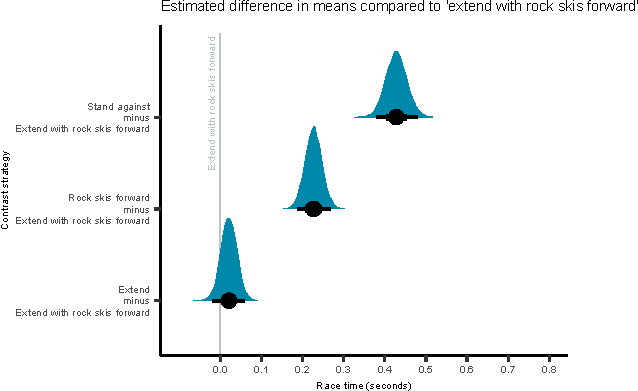
\includegraphics{figure_results_Q1_strategies.pdf}
\caption{Estimated differences in means compared to 'extend with rock skis forward'. The circle represents the point estimates whereas the shaded distribution represents the posterior distribution fitted from the model}
\label{fig:q1_strategieseffect}
\end{figure}

\subsection{Why do they perform better?}


\subsubsection{Contextual interference}







\section{Discussion}

\section{}

\printbibliography

\end{document}
